\chapter{Risuonatori}
\section{Circuito Risonante Serie}
L'\textbf{impedenza} di un \textbf{circuito LC} è la seguente:
\begin{equation*}
    Z = j\w L + \frac{1}{j\w C} = j \sqrt{\frac{L}{C}} \left(\frac{\w}{\w_0}- \frac{\w_0}{\w}\right)
\end{equation*}
dove $\w_0 = \frac{1}{\sqrt{LC}}$ viene detta \textbf{pulsazione di risonanza}, mentre $\sqrt{\frac{L}{C}}$ è il \textbf{parametro di pendenza}.\\ \\
Alla \textbf{pulsazione di risonanza},\textbf{ l'energia elettrica immagazzinata nella capacità eguaglia l'energia magnetica immagazzinata nell'induttore}, quindi:
\begin{equation*}
    Z(\w_0) = 0
\end{equation*}
Invece per pulsazioni prossime a $\w_0$, usando l'approssimazione di \textbf{Taylor}, vale:
\begin{equation*}
    Z \approx j \sqrt{\frac{L}{C}} \frac{2(\w - \w_0)}{\w_0}, \quad \w \approx \w_0
\end{equation*}

\section{Circuito Risonante Parallelo}
Nel caso del \textbf{parallelo} si ragiona con le \textbf{ammettenze}:
\begin{equation*}
    Y = j \w C + \frac{1}{j \w L} = j \sqrt{\frac{C}{L}} \left(\frac{\w}{\w_0} - \frac{\w_0}{\w}\right)
\end{equation*}
Dove $\w_0 = \frac{1}{\sqrt{LC}}$, in corrispondenza della quale vale che $W_E = W_M$.

\section{Circuito Risonante con Perdite}
In un \textbf{circuito risonante reale} vi è una \textbf{resistenza} (conduttanza) che tiene conto delle \textbf{perdite}.\\ \\
Facciamo l'esempio del \textbf{circuito serie}:
\begin{equation*}
    Z =  j \sqrt{\frac{L}{C}} \left(\frac{\w}{\w_0}- \frac{\w_0}{\w}\right) + R_L
\end{equation*}
Definiamo il \textbf{fattore di merito del circuito} come:
\begin{equation*}
    Q = \frac{\w_0 \cdot W_{EM}}{P_{diss}} = \frac{2 \w_0 L \frac{|I|^2}{4}}{\frac{1}{2} R_L |I|^2} = \frac{\w_0 L}{R_L}
\end{equation*}
Così l'\textbf{impedenza} diventa:
\begin{equation*}
    Z = j \sqrt{\frac{L}{C}} \left(\frac{\w}{\w_0} - \frac{\w_0}{\w}\right) + \frac{\w_0 L}{Q} = j \sqrt{\frac{L}{C}} \left(\frac{\w}{\w_0} - \frac{\w_0}{\w} + \frac{1}{j Q}\right)
\end{equation*}
Analogo discorso per il \textbf{parallelo}:
\begin{equation*}
    Y = j \sqrt{\frac{C}{L}} \left(\frac{\w}{\w_0} - \frac{\w_0}{\w}\right) + G = j \sqrt{\frac{L}{C}} \left(\frac{\w}{\w_0} - \frac{\w_0}{\w} + \frac{1}{j Q}\right)
\end{equation*}

\section{Capacità Filtranti di un Risuonatore}
Se colleghiamo un \textbf{risuonatore serie} ad un \textbf{generatore ideale di tensione} a pulsazione $\w$, avremo questa \textbf{corrente}:
\begin{squared}[violet]
    I(\w) = \frac{V_0}{j \sqrt{\frac{L}{C}} \left(\frac{\w}{\w_0} - \frac{\w_0}{\w} + \frac{1}{j Q}\right)}
\end{squared}
Per $\w = \w_0$ la corrente avrà il suo \textbf{massimo}:
\begin{equation*}
    I(\w_0) = V_0 Q \sqrt{\frac{C}{L}}
\end{equation*}
\textbf{A quali pulsazioni il modulo della corrente diminuirà di 3dB??}
\begin{equation*}
    \frac{\w}{\w_0} - \frac{\w_0}{\w} = \pm \frac{1}{j Q}
\end{equation*}
Che ha per soluzioni:
\begin{equation*}
    \w = \pm \frac{1}{2} \left(\frac{\w_0}{Q} \pm \sqrt{\frac{{\w_0}^2}{Q^2} + 4 {\w_0}^2}\right) = \left(\w_0 \sqrt{1 + \frac{1}{4Q^2} } \pm \frac{\w_0}{2Q}\right)
\end{equation*}
Che per $Q >> 1$ fornisce $\w = \pm \left(\w_0 \pm \frac{\w_0}{2Q}\right)$
\\ \\
Analizziamo ora il \textbf{caso di un generatore reale}, con una sua \textbf{resistenza interna} $R_0$:
\begin{equation*}
\begin{aligned}
    Z &= j \sqrt{\frac{L}{C}} \left(\frac{\w}{\w_0} - \frac{\w_0}{\w} + \frac{1}{j Q}\right) + R_0 = j \sqrt{\frac{L}{C}} \left(\frac{\w}{\w_0} - \frac{\w_0}{\w} + \frac{1}{j Q} + \frac{1}{j Q_{ext}}\right ) = \\
    &=j \sqrt{\frac{L}{C}} \left(\frac{\w}{\w_0} - \frac{\w_0}{\w}  + \frac{1}{j Q_{tot}}\right )
\end{aligned}
\end{equation*}
Dove:
\begin{equation*}
    Q_{ext} = R_0 \sqrt{\frac{C}{L}}
\end{equation*}
Dunque:
\begin{equation*}
    Q_{tot} = \frac{QQ_{ext}}{Q + Q_{ext}} = \left(\frac{1}{Q} + \frac{1}{Q_{ext}}\right)^{-1}
\end{equation*}
Quindi si avrà:
\begin{squared}[violet]
     I(\w) = \frac{V_0}{j \sqrt{\frac{L}{C}} \left(\frac{\w}{\w_0} - \frac{\w_0}{\w} + \frac{1}{j Q_{tot}}\right)}
\end{squared}
\begin{equation*}
    I(\w_0) = V_0 Q_{tot} \sqrt{\frac{C}{L}}
\end{equation*}
E analogamente a prima, \textbf{la pulsazione a 3dB sarà}:
\begin{equation*}
    \w_{3dB} = \pm \frac{\w_0}{2Q_{tot}}
\end{equation*}
\section{Risuonatori a Parametri Distribuiti}
Consideriamo la seguente situazione e poniamo l'origine su uno dei due corti:
\begin{center}
    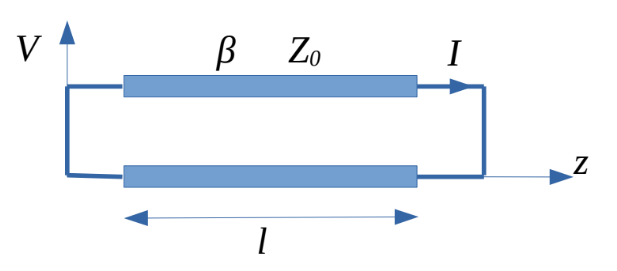
\includegraphics[width=.8\textwidth]{Images/figure28.png}
\end{center}
Avremo i seguenti andamenti di \textbf{tensione} e \textbf{correnti}:
\begin{equation*}
    \begin{dcases}
    V(z) = - j Z_0 I(0) sin(kz)\\
    I(z) = I(0) cos(kz)
    \end{dcases}
\end{equation*}
Mentre l'\textbf{impedenza} sarà:
\begin{equation*}
    Z(z) = - j Z_0 tan(kz) \implies Z(l) = - j Z_0 tan(kl) = Z_R
\end{equation*}
La \textbf{pulsazione di risonanza} è quella in cui $Z = 0$, quindi:
\begin{equation*}
\begin{aligned}
    Z(l) &=  - j Z_0 tan(kl) = 0 \implies tan(\beta l - j \alpha l) \approx \\
    &\approx  tan(\beta l) + \frac{1}{cos^2(\beta l) (-j \alpha l)}
\end{aligned}
\end{equation*}
\textbf{Se le perdite sono piccole} allora:
\begin{equation*}
    \alpha l << 1
\end{equation*}
Quindi:
\begin{equation*}
    Z_R = j Z_0 tan(kl) \approx j Z_0 tan(\beta l) + \frac{Z_0}{cos^2(\beta l)} \alpha l
\end{equation*}
Quindi le\textbf{ pulsazioni di risonanza} sono:
\begin{equation*}
    \w_n: \quad \beta(\w_n) l = (n+1)\pi, \quad n \in N_0
\end{equation*}
In corrispondenza delle quali:
\begin{equation*}
    Z_R = Z_0 \alpha l
\end{equation*}
Quindi ci sono estreme differenze tra \textbf{risuonatori} a \textbf{parametri} \textbf{concentrati} e quelli \textbf{distribuiti}.\\ \\
In un \textbf{risuonatore a parametri concentrati} si ha \textbf{un solo valore di pulsazione di risonanza}, mentre nei \textbf{risuonatori a parametri distribuiti} se ne hanno \textbf{infiniti}.\\ \\
In comune hanno che \textbf{entrambe le impedenze si annullano in risonanza}.\\ \\
Altre analogie le possiamo trovare se analizziamo il comportamento dei due risuonatori in un intorno di ${\w_0}_{(n)}$.\\
Assumiamo che entrambi i \textbf{risuonatori} risuonino a:
\begin{equation*}
    \w_0 = \frac{\pi}{\beta(\w_0)l}
\end{equation*}
Sviluppiamo le due impedenze al primo ordine di \textbf{Taylor}:\footnote{$f(x_0) + \frac{1}{1!}f'(x_0) (x-x_0) $}
\begin{equation*}
    Z'_R \approx \sqrt{\frac{L_0}{C_0}} \left(\frac{\w- \w_0}{2\w_0} - j \frac{1}{Q}\right)
\end{equation*}
\begin{equation*}
    Z_R \approx j Z_0 l \left[\frac{d\beta}{d \w}\right]_{\w=\w_0} (\w - \w_0) + \underbrace{Z_0 \alpha l}_{f(x_0)}
\end{equation*}
Che coincidono se:
\begin{equation*}
    \sqrt{\frac{L_0}{C_0}} = \w_0 \frac{Z_0 l}{2} \left[\frac{d\beta}{d \w}\right]_{\w=\w_0}
\end{equation*}
E se:
\begin{equation*}
    Q = \frac{\w_0}{2\alpha} \left(\left[\frac{d\beta}{d \w}\right]_{\w=\w_0}\right)^{-1}
\end{equation*}
\subsection{Metodo Perturbativo}
Un altro metodo di valutazione è \textbf{l'analisi delle perturbazioni}.\\ \\
Consideriamo una linea \textbf{non dispersiva}, ovvero con i parametri L, R, C, G \textbf{indipendenti} dalla frequenza:
\begin{equation*}
    Z_R = j Z_0 tan(\beta l)
\end{equation*}
\begin{equation*}
    \beta(\w_0) l = (n + 1) \pi, \quad n \in N_0
\end{equation*}
Sviluppiamo $Z_R$ al\textbf{ primo ordine} in $(\w -\w_0) $ e valutiamone il\textbf{ fattore di pendenza}:
\begin{equation*}
    \w_0 \frac{Z_0 l}{2}  \left[\frac{d\beta}{d \w}\right]_{\w=\w_0} = \frac{\w_0 Z_0 l \sqrt{LC}}{2}
\end{equation*}
Per valutare Q scriviamo \textbf{tensione} e \textbf{corrente} lungo la linea:
\begin{equation*}
    \begin{dcases}
    V(z) = V(0) cos(\beta z) = V(0) cos(\pi/l z)\\
    I(z) = - j \frac{V(0)}{Z_0} sin(\beta z) = - j \frac{V(0)}{Z_0} sin(\pi/l z)
    \end{dcases}
\end{equation*}
Essendo la linea \textbf{non dispersiva}, calcoliamo $W_E$ e $W_M$ come:
\begin{equation*}
    \begin{dcases}
    W_E = \frac{1}{4} C \int_l |V(z)|^2 dz\\
    W_M = \frac{1}{4} L \int_l |I(z)|^2 dz
    \end{dcases}
\end{equation*}
E le \textbf{potenze dissipate} come:
\begin{equation*}
    \begin{dcases}
    P_R = \frac{1}{2} R \int_l |I(z)|^2 dz\\
    P_G = \frac{1}{2} G \int_l |V(z)|^2 dz
    \end{dcases}
\end{equation*}
E infine calcolo Q:
\begin{equation*}
\begin{aligned}
    Q &= \frac{\w_0 (W_E + W_M)}{P_R + P_G} = \frac{\w_0 \w_{EM}}{P_R + P_G} = \left(\frac{P_R}{\w_0 \w_{EM}} + \frac{P_G}{\w_0 \w_{EM}} \right)^{-1} = \\
    &=\left(\frac{R}{\w_0 L} + \frac{G}{\w_0 C}\right)^{-1} 
\end{aligned}
\end{equation*}


\section{Esempi di Calcolo di Q in circuiti a parametri Distribuiti}
\subsection{Esempio 1}
Consideriamo la seguente \textbf{linea con piccole perdite} chiusa in \textbf{corto} su entrambe le porte:

\begin{center}
    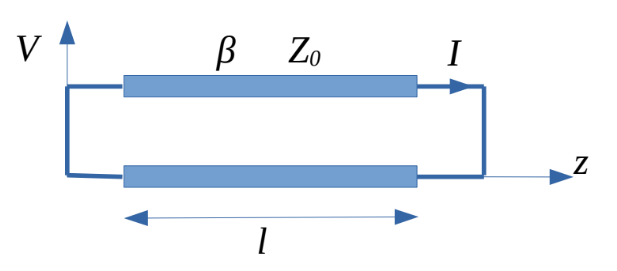
\includegraphics[width=.8\textwidth]{Images/figure28.png}
\end{center}
La linea avrà \textbf{piccole perdite} se:
\begin{itemize}
    \item $\frac{R}{\w L} << 1$\\
    \item $\frac{G}{\w C} << 1$
\end{itemize}
Calcoliamo la \textbf{pulsazione di risonanza fondamentale} e il \textbf{Q} corrispondente:
\begin{equation*}
    \begin{dcases}
    V(z) = - j I(0) Z_0 sin(\beta z)\\
    I(z) = I(0) cos(\beta z)
    \end{dcases}
\end{equation*}
Dove:
\begin{itemize}
    \item $\beta = \w \sqrt{LC}$\\
    \item $Z_0 = \sqrt{\frac{L}{C}}$
\end{itemize}
Quindi:
\begin{equation*}
    \w_0 \sqrt{LC} l = \pi \implies \w_0 = \frac{\pi}{\sqrt{LC} l}
\end{equation*}
Mentre Q sarà:
\begin{equation*}
    Q = \frac{\w_0 W_{EM}}{P_{diss}} = \frac{\w_0 W_{EM}}{P^R_{diss}+ P^G_{diss}} \implies Q = \left(\frac{1}{Q_R} + \frac{1}{Q_G}\right)^{-1}
\end{equation*}
In particolare:
\begin{equation*}
    Q_R = \frac{\w_0 W_{EM}}{P^R_{diss}}, \quad Q_G = \frac{\w_0 W_{EM}}{P^G_{diss}}
\end{equation*}
Dove:
\begin{equation*}
    P^R_{diss} = \frac{1}{2} \int_0^l |I(z)|^2 dz, \quad P^G_{diss} = \frac{1}{2} \int_0^l |V(z)|^2 dz
\end{equation*}.
Quindi:
\begin{equation*}
    W_{EM} = W_M + W_E = \frac{1}{4} L \int_0^l |I(z)|^2 dz + \frac{1}{4} C \int_0^l |V(z)|^2 dz
\end{equation*}
In risonanza $W_E = W_M$, quindi:
\begin{equation*}
    W_{EM} = 2W_M = \frac{1}{2} L \int_0^l |I(z)|^2 dz = \frac{1}{2} C \int_0^l |V(z)|^2 dz = 2W_E
\end{equation*}
Quindi ci\textbf{ semplifichiamo il calcoli} facendo scelte opportune:
\begin{equation*}
    Q_R = \frac{\w_0 \frac{1}{2} L \int_0^l |I(z)|^2 dz}{\frac{1}{2} R \int_0^l |I(z)|^2 dz} = \frac{\w_0 L}{R}
\end{equation*}
\begin{equation*}
    Q_G = \frac{\w_0 \frac{1}{2} C \int_0^l |V(z)|^2 dz}{\frac{1}{2} G \int_0^l |V(z)|^2 dz} = \frac{\w_0 C}{G}
\end{equation*}
Quindi avremo:
\begin{equation*}
    Q = \left(\frac{R}{\w_0 L}  + \frac{G}{\w_0 C}\right)^{-1} = \frac{\w_0 LC}{R C + L G}
\end{equation*}

\subsection{Esempio 2}
Consideriamo la seguente \textbf{linea chiusa su due resistenze, senza perdite}:
\begin{center}
    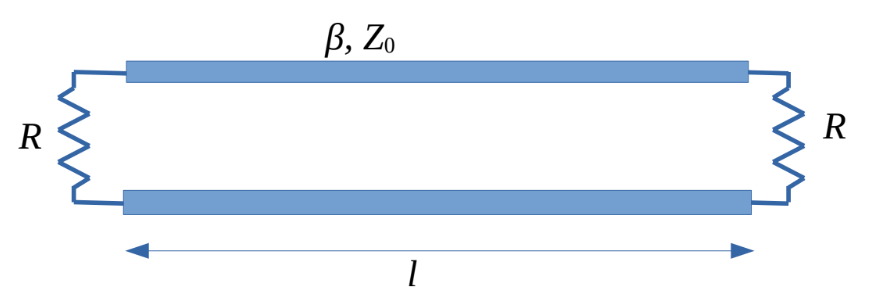
\includegraphics[width=.8\textwidth]{Images/figure29.png}
\end{center}
Suppongo \textbf{R piccole} in modo tale da \textbf{non variare tensioni e correnti sulla linea rispetto al caso 1}.\\ \\
\begin{equation*}
    \begin{dcases}
    V(z) = -j I(0) Z_0 cos(\beta z)\\
    I(z) = I(0) cos(\beta z) 
    \end{dcases}
\end{equation*}
E la \textbf{pulsazione di risonanza} è:
\begin{equation*}
    \w_0\sqrt{LC} l = \pi \implies \w_0 = \frac{\pi}{\sqrt{LC} l }
\end{equation*}
Per calcolare Q ci occorrono l'\textbf{energia immagazzinata e la potenza dissipata}:
\begin{equation*}
    P_{diss} = \frac{1}{2} R |I(0)|^2 + \frac{1}{2} R |I(l)|^2 = R |I(0)|^2
\end{equation*}
\begin{equation*}
\begin{aligned}
    W_{EM} &= 2W_M = \frac{1}{2} L |I(0)|^2 \int_0^l cos^2(\beta z) dz \\
    &(\theta = \beta z \implies dz = \frac{1}{\beta} d\theta)\\
    &\implies \frac{1}{\beta} \int_0^\pi cos^2(\theta) d\theta = \frac{1}{\beta} \int_0^\pi \frac{1}{2} + \frac{1}{2} cos(2\theta) d\theta =\\
    &= \frac{\pi}{2\beta} = \frac{\pi}{2\w_0 \sqrt{LC}} = \frac{\lambda}{4}
\end{aligned}
\end{equation*}
Per cui:
\begin{equation*}
    W_{EM} = \frac{1}{2} L |I(0)|^2 \frac{\pi}{2\w_0 \sqrt{LC}} = \frac{1}{4} \sqrt{\frac{L}{C}} |I(0)|^2 \frac{\pi}{\w_0}
\end{equation*}
Quindi:
\begin{equation*}
    Q = \frac{\w_0 W_{EM}}{P_{diss}} = \frac{\w_0 \frac{1}{4} \sqrt{\frac{L}{C}} |I(0)|^2 \frac{\pi}{\w_0}}{R^2 |I(0)|^2} = \sqrt{\frac{L}{C}} \frac{\pi}{4R} = \frac{\pi}{4} \frac{Z_0}{R}
\end{equation*}
Di conseguenza:
\begin{equation*}
    Q >> 1 \quad se \quad Z_0 >> R
\end{equation*}

\subsection{Esempio 3}
Nel caso in cui $Z_0 << R$, gli andamenti di V e I, sono gli stessi di una \textbf{linea aperta}:
\begin{center}
    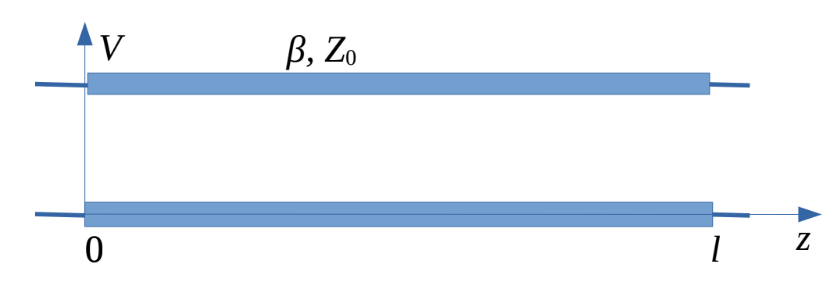
\includegraphics[width=.8\textwidth]{Images/figure30.png}
\end{center}
\begin{equation*}
    \begin{dcases}
    V(z) = V(0) cos(\beta z)\\
    I(z) = -j \frac{V(0)}{Z_0} sin(\beta z)
    \end{dcases}
\end{equation*}
\begin{equation*}
    \w_0 \sqrt{LC} l = \pi \implies \w_0 = \frac{\pi}{\sqrt{LC} l}
\end{equation*}
\begin{equation*}
    P_{diss} = \frac{1}{2} \frac{|V(0)|^2}{R} + \frac{1}{2} \frac{|V(l)|^2}{R} = G|V(0)|^2
\end{equation*}
\begin{equation*}
\begin{aligned}
    W_{EM} &= 2W_E = \frac{1}{2} C |V(0)|^2 \int_0^l cos^2(\beta l) dz = \frac{1}{2} C |V(0)|^2 \frac{\pi}{2\w_0 \sqrt{LC}} = \\
    &=\frac{1}{4} \sqrt{\frac{C}{L}} |V(0)|^2 \frac{\pi}{\w_0}
\end{aligned}
\end{equation*}
Infine:
\begin{equation*}
    Q = \frac{\w_0 W_{EM}}{P_{diss}} = \frac{\w_0 \frac{1}{4} \sqrt{\frac{C}{L}} \frac{\pi}{\w_0}} {G|V(0)|^2} =\sqrt{\frac{C}{L}} \frac{\pi}{4G} = \frac{\pi}{4} \frac{R}{Z_0}
\end{equation*}
Quindi:
\begin{equation*}
    Q >> 1 \quad se \quad Z_0 << R
\end{equation*}

\section{Condizioni di Risonanza su una Rete Complessa}
Consideriamo una rete di \textbf{elementi} \textbf{concentrati} e \textbf{distribuiti} \textbf{senza perdite} e \textbf{senza generatori} e individuiamo una sezione che la divide in due, e alla quale posso inserire un \textbf{generatore di tensione}:
\begin{center}
    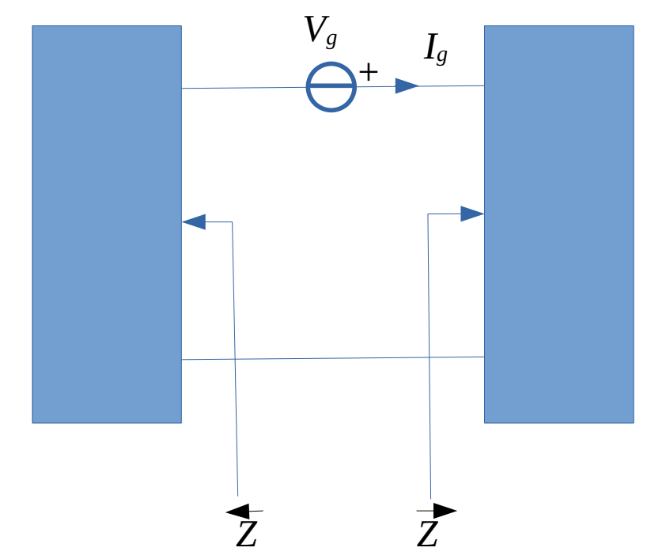
\includegraphics[width=.5\textwidth]{Images/figure31.png}
\end{center}
O di corrente:
\begin{center}
    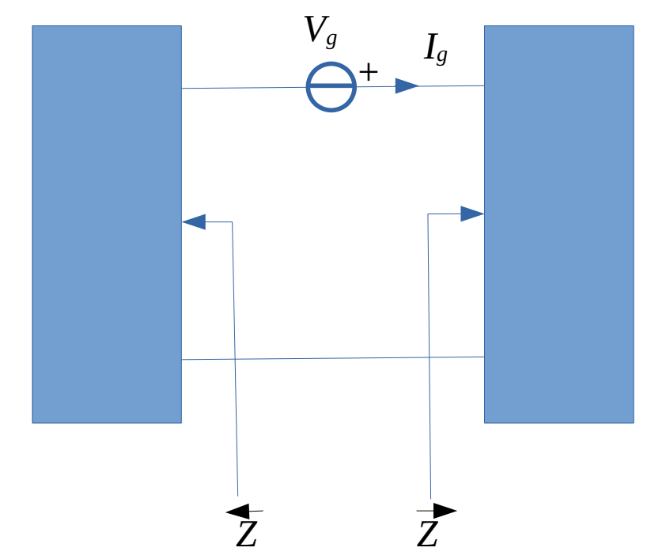
\includegraphics[width=.5\textwidth]{Images/figure31.png}
\end{center}
Nel primo caso:
\begin{equation*}
    I = \frac{V_G}{\overleftarrow{Z}\overrightarrow{Z}}
\end{equation*}
Dove le due impedenze sono pure \textbf{reattanze}.\\ \\
Può accadere che a qualche frequenza $\overleftarrow{Z} + \overrightarrow{Z} = 0$ e nel caso in cui anche $V_G$ fosse 0, queste frequenze vengono dette di \textbf{risonanza}. \\ \\
In modo analogo:
\begin{equation*}
    V = \frac{I_G}{\overleftarrow{Y}\overrightarrow{Y}}
\end{equation*}
Se $\overleftarrow{Y} + \overrightarrow{Y} = 0$ e  $I_G = 0$ sono dette \textbf{frequenze di risonanza}.\\ \\
\begin{center}
    Devono valere entrambe.
\end{center}

\subsection{Esempio 1}
\begin{center}
    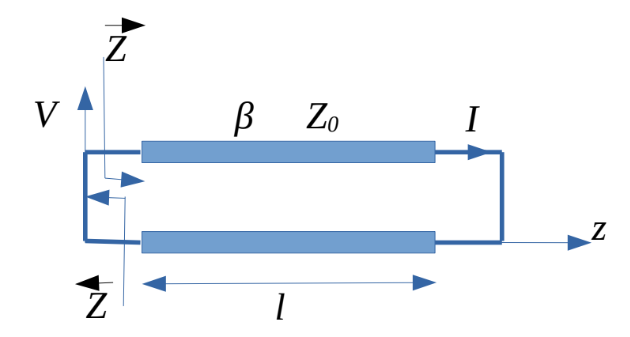
\includegraphics[width=.5\textwidth]{Images/figure33.png}
\end{center}
\begin{equation*}
    \overleftarrow{Z} + \overrightarrow{Z} = 0 + j Z_0 tan(\beta l) = 0
\end{equation*}
\begin{equation*}
    \implies \beta l = n\pi
\end{equation*}
Ma in questo caso:
\begin{equation*}
    \overleftarrow{Y} \longrightarrow \infty
\end{equation*}
\textbf{Quindi non va bene.}
\subsection{Esempio 2}
\begin{center}
    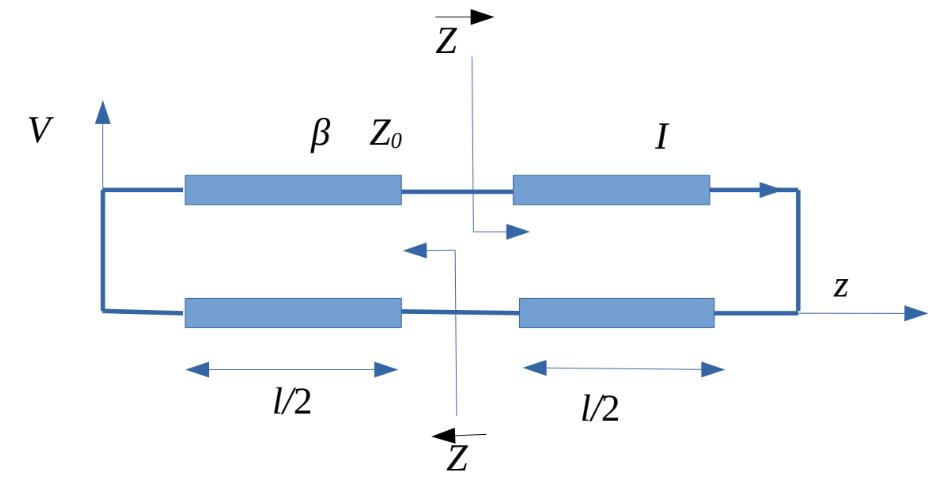
\includegraphics[width=.5\textwidth]{Images/figure34.png}
\end{center}
\begin{equation*}
    \overleftarrow{Z} + \overrightarrow{Z} = j Z_0 tan(\beta l/2) + j Z_0 tan(\beta l/2) = 2 j Z_0 tan(\beta l/2) = 0
\end{equation*}
Le cui soluzioni sono:
\begin{equation*}
    \beta  \frac{l}{2} = \frac{n}{\pi} \leftrightarrow \beta l = 2n\pi \implies l = 2n\frac{\lambda}{2} = n \lambda
\end{equation*}
Mentre per le \textbf{ammettenze}:
\begin{equation*}
    \overleftarrow{Y} + \overrightarrow{Y} = - j Y_0 tan(\beta l/2) - j Y_0 cotan(\beta l/2) = - 2 j Y_0 cotan(\beta l/2) = 0
\end{equation*}
Le cui soluzioni sono:
\begin{equation*}
    \beta  \frac{l}{2} = \frac{\pi}{2} + n\pi \leftrightarrow \beta l = (2n+1) \pi \implies l = (2n+1) \frac{\lambda}{2} 
\end{equation*}
\textbf{Quindi va bene!!}